\section{نتایج نسخه استاندارد}
\label{sec:std_results}
در این بخش، نتایج نسخه‌های تک‌عاملی الگوریتم‌ها در سناریوهای مقاومت مختلف ارائه و تحلیل می‌شود.

\subsection{توزیع پاداش تجمعی}
\begin{figure}[H]
	\centering
	
	% سطر اول
	\subfloat[شرایط اولیه تصادفی]{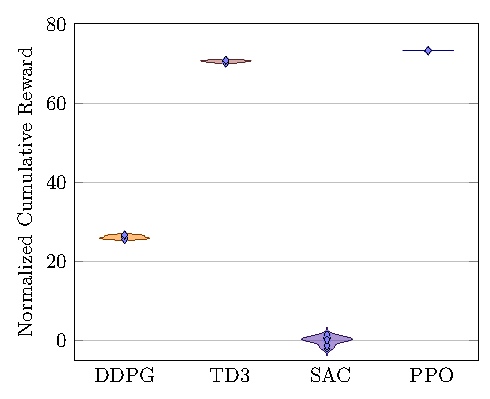
\includegraphics[width=.33\textwidth]{plots/standard/violin_plot/initial_condition_shift.pdf}}%
	\subfloat[اغتشاش در عملگرها]{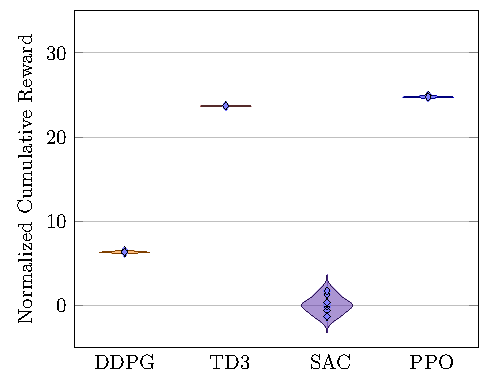
\includegraphics[width=.33\textwidth]{plots/standard/violin_plot/actuator_disturbance.pdf}}%
	\subfloat[عدم تطابق مدل]{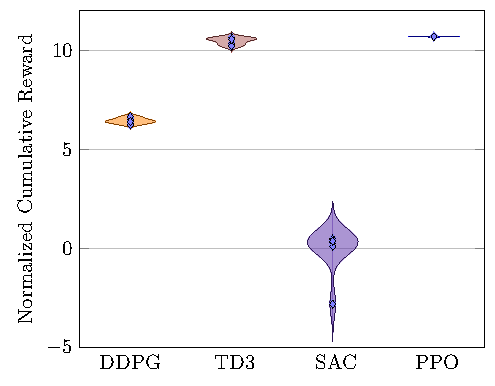
\includegraphics[width=.33\textwidth]{plots/standard/violin_plot/model_mismatch.pdf}}\\[1ex]
	
	% سطر دوم
	\subfloat[مشاهده ناقص]{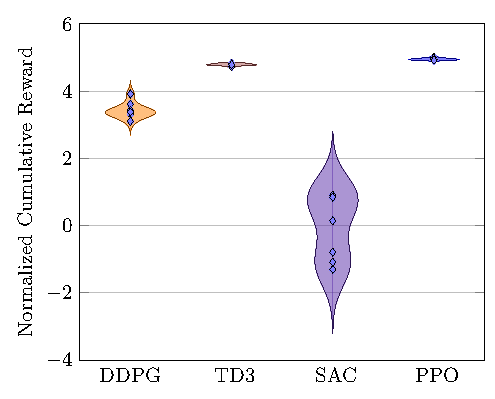
\includegraphics[width=.33\textwidth]{plots/standard/violin_plot/partial_observation.pdf}}%
	\subfloat[نویز حسگر]{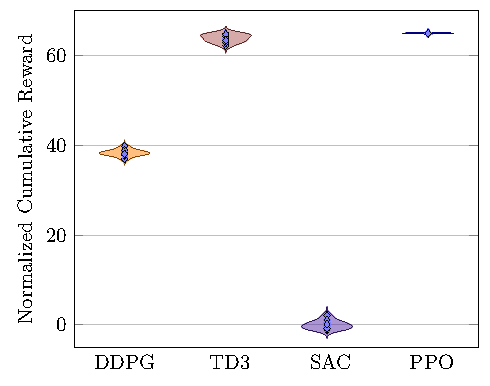
\includegraphics[width=.33\textwidth]{plots/standard/violin_plot/sensor_noise.pdf}}%
	\subfloat[تأخیر زمانی]{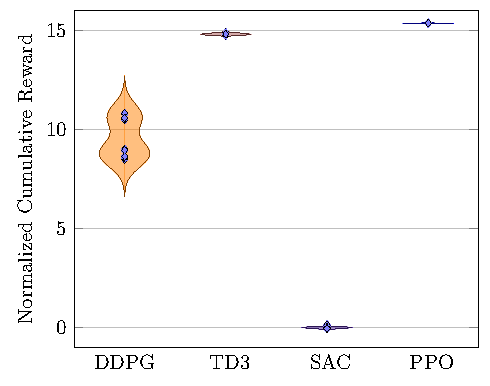
\includegraphics[width=.33\textwidth]{plots/standard/violin_plot/time_delay.pdf}}
	
	\caption{مقایسه توزیع پاداش تجمعی برای نسخه‌های تک‌عاملی  در سناریوهای مختلف.}
	\label{fig:std_robustness_violin}
\end{figure}

\subsection{مقایسه عددی}
\begin{table}[H]
	\centering
	\setlength{\tabcolsep}{6pt}
	\renewcommand{\arraystretch}{1.5}
	\scriptsize
	
	% --- Row 1: left + right boxes, centered as a group ---
	\makebox[\linewidth][c]{%
		\parbox{.48\linewidth}{
			\centering
			\footnotesize
			\begin{tabular}{@{} R {2.6cm}*{4}{c}}
				\toprule
				{سناریو} & \lr{DDPG} & \lr{PPO} & \lr{SAC} & \lr{TD3} \\
				\midrule
				شرایط اولیه تصادفی & $-0.27$ & $0.61$ & $-0.76$ & $0.56$ \\
				اغتشاش در عملگرها & $-0.38$ & $0.61$ & $-0.72$ & $0.55$ \\
				عدم تطابق مدل      & $-0.84$ & $0.58$ & $-2.98$ & $0.51$ \\
				مشاهده ناقص        & $-0.88$ & $0.36$ & $-3.65$ & $0.23$ \\
				نویز حسگر          & $-0.85$ & $0.58$ & $-2.90$ & $0.52$ \\
				تأخیر زمانی        & $-0.76$ & $0.61$ & $-2.98$ & $0.48$ \\
				\bottomrule
			\end{tabular}
			\caption*{\normalfont پاداش تجمعی}
		}
		\hspace{0.04\linewidth}
		\parbox{.48\linewidth}{
			\centering
			\footnotesize
			\begin{tabular}{@{} R {2.6cm}*{4}{c}}
				\toprule
				{سناریو} & \lr{DDPG} & \lr{PPO} & \lr{SAC} & \lr{TD3} \\
				\midrule
				شرایط اولیه تصادفی & $3.30$ & $2.56$ & $8.06$ & $0.72$ \\
				اغتشاش در عملگرها & $3.74$ & $2.58$ & $7.91$ & $0.77$ \\
				عدم تطابق مدل      & $10.87$ & $3.06$ & $17.12$ & $1.09$ \\
				مشاهده ناقص        & $8.18$ & $3.34$ & $15.47$ & $1.77$ \\
				نویز حسگر          & $11.04$ & $3.08$ & $16.81$ & $1.02$ \\
				تأخیر زمانی        & $8.95$ & $2.27$ & $15.70$ & $0.81$ \\
				\bottomrule
			\end{tabular}
			\caption*{\normalfont مجموع خطای مسیر}
		}%
	}
	
	\vspace{0.6em}
	
	% --- Row 2: left + right boxes, centered as a group ---
	\makebox[\linewidth][c]{%
		\parbox{.48\linewidth}{
			\centering
			\footnotesize
			\begin{tabular}{@{} R {2.6cm}*{4}{c}}
				\toprule
				{سناریو} & \lr{DDPG} & \lr{PPO} & \lr{SAC} & \lr{TD3} \\
				\midrule
				شرایط اولیه تصادفی & $5.11$ & $0.77$ & $1.76$ & $3.31$ \\
				اغتشاش در عملگرها & $4.89$ & $0.77$ & $1.71$ & $3.07$ \\
				عدم تطابق مدل      & $5.48$ & $0.86$ & $2.37$ & $4.32$ \\
				مشاهده ناقص        & $5.37$ & $1.03$ & $2.33$ & $4.10$ \\
				نویز حسگر          & $5.48$ & $0.86$ & $2.37$ & $4.30$ \\
				تأخیر زمانی        & $5.51$ & $0.76$ & $2.11$ & $5.12$ \\
				\bottomrule
			\end{tabular}
			\caption*{\normalfont مجموع تلاش کنترلی}
		}
		\hspace{0.04\linewidth}
		\parbox{.48\linewidth}{
			\centering
			\footnotesize
			\begin{tabular}{@{} R {2.6cm}*{4}{c}}
				\toprule
				{سناریو} & \lr{DDPG} & \lr{PPO} & \lr{SAC} & \lr{TD3} \\
				\midrule
				شرایط اولیه تصادفی & $0.00$ & $0.00$ & $0.00$ & $0.00$ \\
				اغتشاش در عملگرها & $0.00$ & $0.00$ & $0.00$ & $0.00$ \\
				عدم تطابق مدل      & $0.00$ & $0.00$ & $1.00$ & $0.00$ \\
				مشاهده ناقص        & $0.00$ & $0.00$ & $1.00$ & $0.00$ \\
				نویز حسگر          & $0.00$ & $0.00$ & $1.00$ & $0.00$ \\
				تأخیر زمانی        & $0.00$ & $0.00$ & $1.00$ & $0.00$ \\
				\bottomrule
			\end{tabular}
			\caption*{\normalfont احتمال شکست}
		}%
	}
	
	\caption{مقایسه الگوریتم‌های چندعاملی در سناریوهای مختلف مقاومت}
\end{table}


%\subsection{تحلیل و بحث}
بر اساس داده‌ها، \lr{TD3} به‌طور پایدار بالاترین پاداش و کمترین خطای مسیر را ثبت می‌کند، درحالی‌که \lr{PPO} کمترین تلاش کنترلی را دارد. \lr{SAC} در برخی سناریوهای دشوار (عدم تطابق مدل، مشاهده ناقص، نویز حسگر، تأخیر زمانی) نرخ شکست بالاتری نشان می‌دهد و \lr{DDPG} عموماً از نظر پاداش و خطا ضعیف‌تر از \lr{PPO} و \lr{TD3} است.

